\chapter{Introduction non facultative}\label{chapIntro}

Ce chapitre présente les besoins et les concepts de la gestion de
versions d'une manière générale, ainsi qu'un aperçu des différentes
familles de systèmes de gestion de versions. Il se focalise ensuite sur
Git, qui sera l'objet du reste de cet ouvrage, pour en expliquer la
philosophie et le modèle de fonctionnement.

\section{Les besoins du génie logiciel}

La \textbf{gestion de versions}\index{Gestion de versions} (en anglais
\textit{version control} ou \textit{revision control}) est une
fonctionnalité, ou plutôt une famille de fonctionnalités, qui trouve
son origine dans les besoins du développement logiciel en
équipe. Plusieurs développeurs travaillant ensemble sur le même
ensemble de fichiers, même si les domaines d'intervention de chacun
sont clairement définis, doivent nécessairement trouver un moyen de
collaborer de manière constructive, sans que les contributions des uns
ne deviennent un souci pour les autres. La gestion de version, en
s'appuyant sur un \textbf{historique}\index{historique} raisonné du
développement, a pour vocation de répondre à l'ensemble des besoins
détaillés ci-après.

\subsection{Gestion des instances du projet}

Les outils de gestion de versions doivent permettre d'identifier
plusieurs instances (éventuellement à des stades de développement
différents) du même projet. Ces instances peuvent correspondre,
suivant les cas, à l'espace de travail direct d'un développeur ou d'un
ensemble de développeurs, à une instance de référence commune partagée
par tous ou par un sous-groupe des développeurs, à une instance de
mise à disposition du public des versions stables du projet\ldots

Ces instances sont désignées sous le terme générique de
\textbf{dépôt}\index{depot@dépôt} (\textit{repository} en
anglais). Chaque dépôt est une représentation du projet. Suivant les
choix d'organisation et le système de gestion de versions utilisé, un
dépôt peut représenter le projet dans son intégralité ou bien
seulement un sous-ensemble, l'intégralité de son historique ou bien
seulement une partie. Un dépôt peut être
\textbf{local}\index{depot@dépôt!local}, c'est-à-dire situé sur la
machine de développement d'un des contributeurs (sans être
nécessairement confondu avec l'espace de travail direct du
développeur), ou bien \textbf{distant}\index{depot@dépôt!distant},
déporté sur un serveur accessible via le réseau.

\subsection{Gestion de l'historique}

La gestion de versions est un moyen de conserver une trace de
l'historique du projet (ou plus précisément d'un dépôt), sous la forme
d'un ensemble de \textbf{révisions}\index{revision@révision}
(\textit{commits} en anglais). Une révision est un ensemble atomique
et identifiable de modifications liées par une certaine unité
sémantique, portant sur un ou plusieurs fichiers, réalisées par un
même contributeur identifié, explicitement introduites dans le projet,
accompagnées d'un message explicatif et d'autres méta-données, comme
la date\footnote{Dans certains systèmes, comme par exemple
  Overleaf\index{Overleaf}, qui est une surcouche web de Git pour la
  rédaction collaborative (\url{https://www.overleaf.com/}), les
  révisions peuvent être générées automatiquement, de manière
  périodique ou à chaque modification élémentaire. Dans ce cas, une
  révision peut n'avoir ni unité sémantique ni message explicatif, ce
  qui limite forcément l'utilité de l'historique résultant. D'autre
  part, l'unicité sémantique des révisions est une propriété qui, si
  elle est désirable, dépend en grande partie de la bonne volonté des
  contributeurs\ldots}. L'atomicité signifie que les modifications
d'une même révision sont toutes appliquées ensemble au projet (ou
qu'aucune ne l'est), sans qu'une modification provenant d'une autre
révision puisse venir interférer ni que le projet puisse se retrouver
dans un état incohérent (avec une révision partiellement
appliquée)\footnote{Il existe des systèmes de gestion de versions dans
  lesquels les révisions ne sont pas atomiques. Nous ne les
  mentionneront pas ici, dans l'espoir que leur nom disparaisse à
  jamais de la mémoire collective et de l'histoire de l'informatique
  (pour plus de détails sur les bonnes pratiques du révisionnisme avec
  Git, les nostalgiques du Ministère de la Vérité \cite{Orwell}
  pourront étudier avec intérêt la section~\ref{secRevisionnisme}).}.
Par abus de langage, le terme de révision ou de \textit{commit}
désigne également l'état du projet après application des modifications
en question.

Dans le cas le plus simple, un historique est une succession linéaire
de révisions, chacune s'appuyant sur la précédente
(figure~\ref{fig:historiqueLineaire}). Dans la majorité des cas,
cependant, il en ira tout autrement\ldots\ Dans la syntaxe graphique
que nous adoptons pour les historiques, les cercles représentent les
révisions et les flèches représentent les dépendances entre
ces révisions. Le sens de ces flèches n'est donc pas le sens d'écoulement
du temps (qui va de la gauche vers la droite pour un historique
linéaire)~: le fait que la révision $E$ pointe vers la révision $D$
($D \leftarrow E$) veut dire que $E$ s'appuie sur $D$, et donc qu'elle
vient après cette dernière dans le processus de conception.

\begin{figure}[h!]
  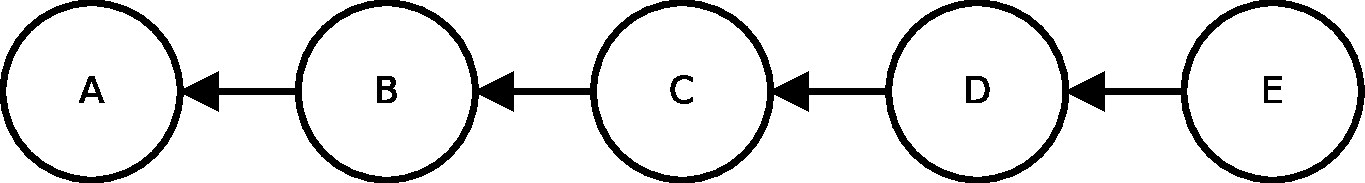
\includegraphics[width=10cm]{figures/historiqueLineaire}
  \caption{Exemple d'historique de développement linéaire, constitué
    de cinq révisions successives.\label{fig:historiqueLineaire}}
\end{figure}


L'historique a lui-même différentes utilités, au-delà de ce rôle de
représentation temporelle, notamment parce qu'il est généralement
navigable, voire cherchable. Suivant les systèmes, l'historique peut
permettre de déterminer~:
\begin{itemize}
\item La date d'introduction d'une révision donnée~;
\item L'auteur d'une révision donnée~;
\item Les modifications apportées par une révision donnée~;
\item Les causes et motivations d'une modification (si la révision
  concernée a été correctement documentée)~;
\item La révision ayant introduit une fonctionnalité, un
  bogue\index{bogue}, une régression\index{regression@régression}, une
  vulnérabilité\ldots
\item \ldots
\end{itemize}

\subsection{Intégration de contributions dans un même projet} % TODO 

Les différentes personnes participant à un même projet doivent pouvoir
voir leurs contributions individuelles intégrées au projet, idéalement
de manière fluide, transparente et indolore. Le problème qui se pose
(et qui est partagé avec nombre d'autres domaines de l'informatique)
est bien évidemment celui de la concurrence entre les
modifications. Si deux développeurs, travaillant sur le même dépôt de
référence, modifient le même fichier, chacun de son côté, comment les
modifications de l'un peuvent-elles être prises en compte sans
impacter négativement (ou oblitérer complètement) le travail de
l'autre au moment d'enregistrer les révisions dans le dépôt~? Si les
deux développeurs souhaitent effectuer des modifications différentes
et jugées incompatibles par le système de gestion de versions, ce
dernier informera de l'existence d'un \textbf{conflit}\index{conflit},
qui devra être résolu avant de pouvoir continuer le développement.

La figure~\ref{fig:conflit} illustre l'apparition d'un conflit dans la
rédaction d'un document. À un certain point, le dépôt contient un
texte affirmant que les continents d'Oceania et d'Estasia sont alliés
depuis toujours dans une guerre contre Eurasia. La connaissance du
contenu de ce document est partagé de toutes les personnes ayant accès
au dépôt. Une évolution de la situation nécessite que le document soit
édité et deux rédacteurs s'attellent simultanément à la tâche, chacun
ignorant l'entreprise de l'autre. Le premier corrige le document pour
lui faire dire qu'Oceania et Eurasia sont alliés depuis toujours dans
une guerre contre Estasia, pendant que le deuxième introduit une
modification différente, reflétant sa propre vision du monde et sa
propre expertise de la
géopolitique\footnote{\url{https://en.wikipedia.org/wiki/Communications_Over_Various_Feeds_Electronically_for_Engagement_Act}.}. Ces
deux révisions traduisent des réalités complètement différentes et,
dans ce cas précis, leurs différences ne peuvent être résolues
automatiquement par un système de gestion de versions. Un conflit
survient lorsque les deux rédacteurs tentent de faire accepter leurs
révisions dans le dépôt\footnote{Le moment exact d'apparition du
  conflit et les possibiltés de résolution correspondantes dépendent
  du modèle utilisé par le système de gestion de versions.}. Un
utilisateur humain (typiquement, l'un des deux contributeurs) doit
alors intervenir pour
\textbf{résoudre}\index{conflit!resolution@résolution} le conflit et
déterminer la version du document devant apparaître dans le dépôt.

\begin{figure}[h!]
  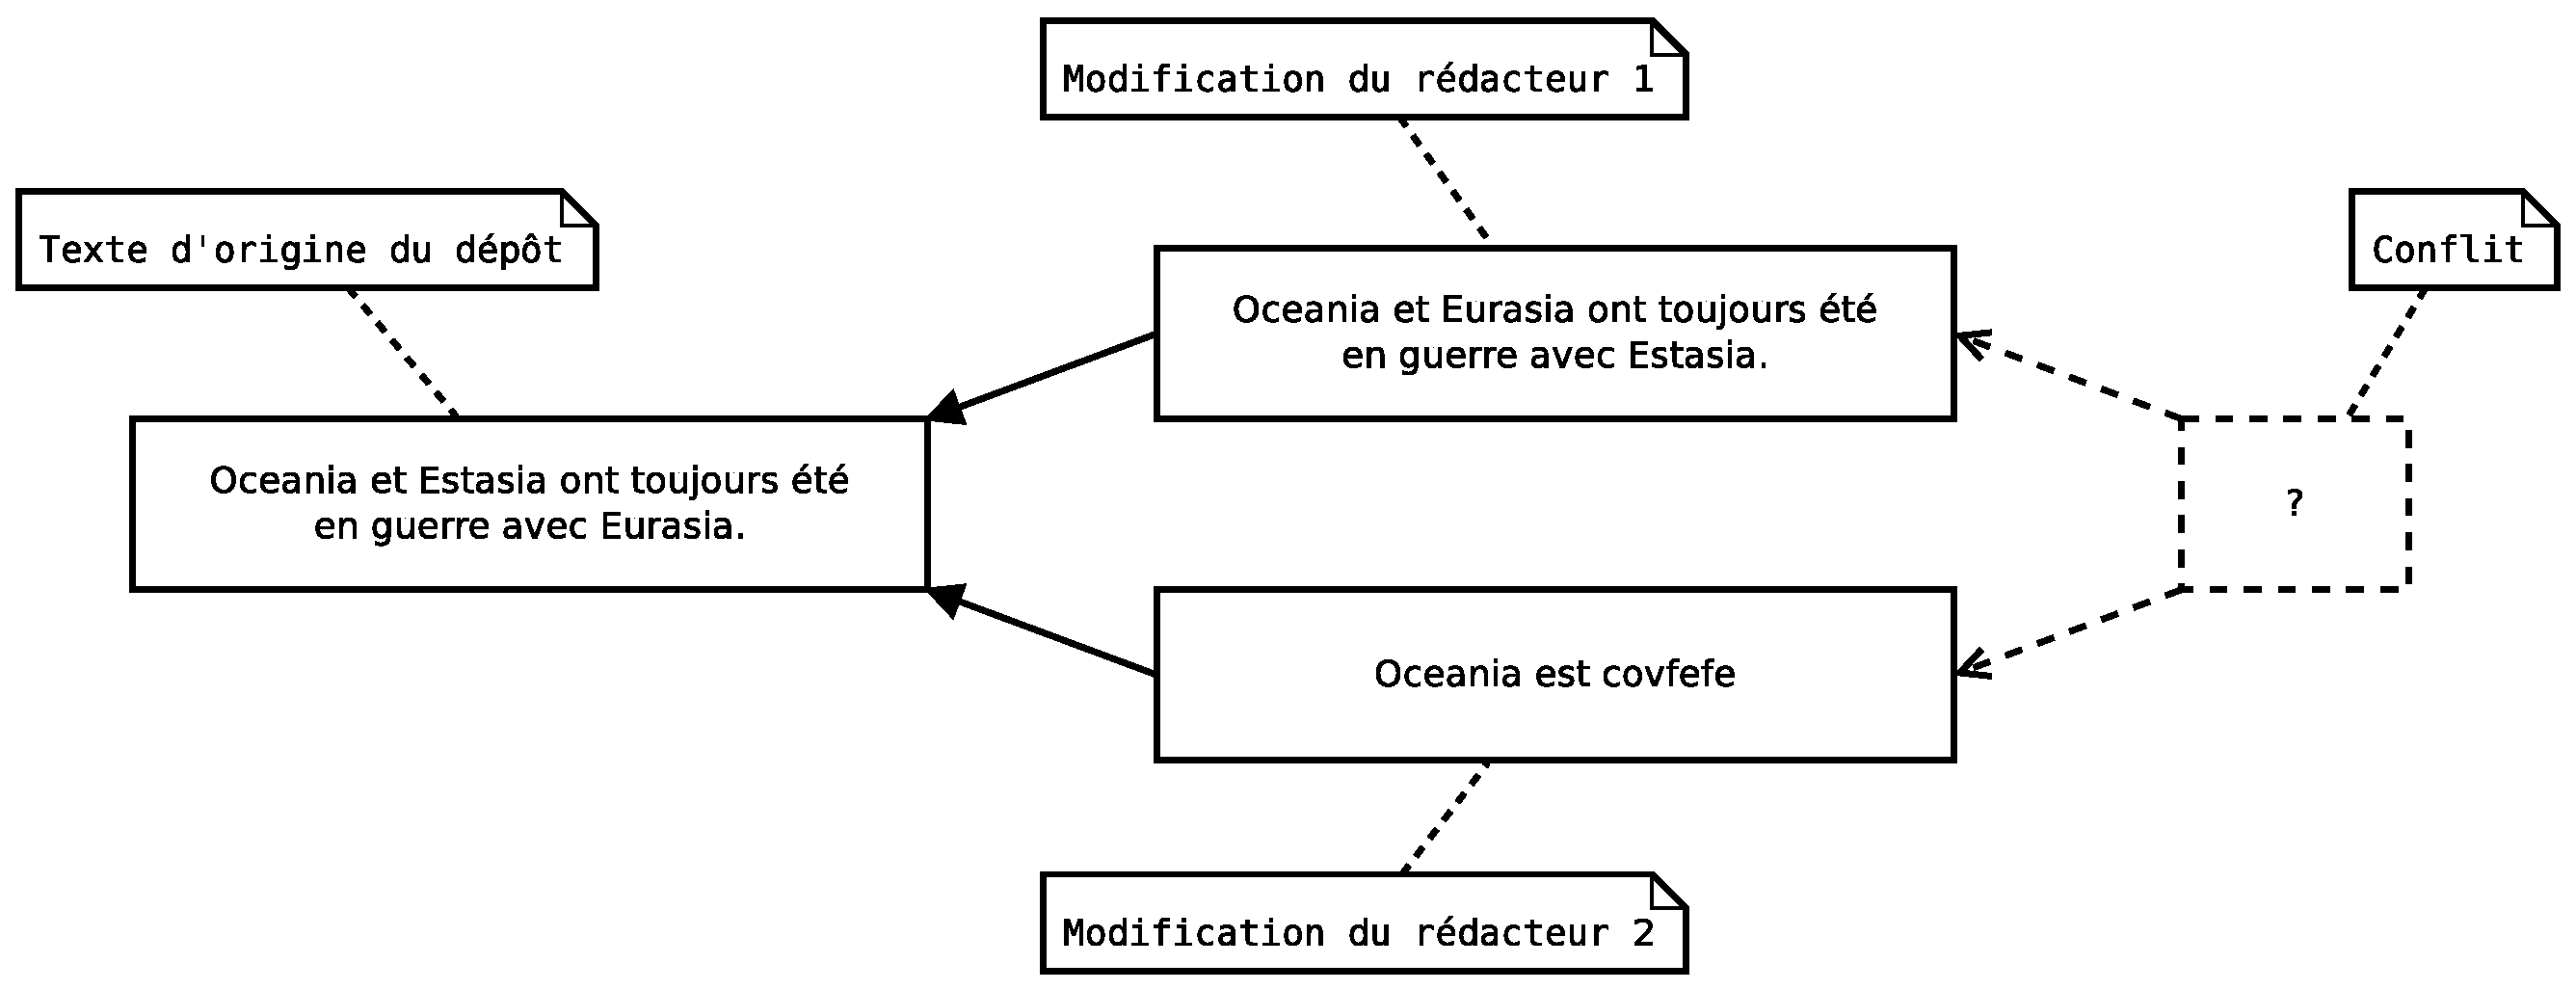
\includegraphics[width=15cm]{figures/conflit}
  \caption{Apparition d'un conflit entre les contributions de deux
    contributeurs.\label{fig:conflit}}
\end{figure}

Une première solution au problème des conflits dans les systèmes de
gestion de versions est le \textbf{verrouillage}\index{verrou} des
fichiers, qui empêche complètement l'apparition des
conflits\footnote{La notion de verrou en informatique est utilisée
  dans de nombreux autres domaines dans lesquels se posent des
  problèmes de concurrence.}. Si l'on applique cette stratégie à notre
scénario, le premier rédacteur déclarera prendre la main sur le
fichier lorsqu'il commencera à travailler dessus. Le système gérant le
dépôt y posera alors un verrou. Le deuxième rédacteur pourra toujours
ouvrir le fichier en lecture, mais aucune modification ne lui sera
possible tant que le premier rédacteur n'aura pas enregistré sa
révision dans le dépôt, relâchant ainsi le verrou. Cette stratégie de
verrouillage est efficace pour éviter les problèmes de concurrence,
mais elle est très contraignante pour le développement en équipe car
elle interdit le travail simultané sur une même portion du
projet. C'est pour cela qu'elle est rarement utilisée comme moyen
principal de gestion des conflits dans les systèmes modernes de
gestion de versions\footnote{La gestion de concurrence par
  verrouillage pose en fait plusieurs types de problèmes
  \cite[chap.~1]{SVNbook}~:
  \begin{itemize}
  \item Il est possible pour un contributeur de prendre un verrou et
    de ne jamais le relâcher (parce qu'il ne valide jamais sa
    révision), nécessitant ainsi l'intervention d'un administrateur
    pour permettre aux autres développeurs de contribuer~;
  \item Des verrous inutiles peuvent être imposés, notamment lorsque
    deux contributeurs souhaitent éditer des parties différentes et
    indépendantes d'un même projet~;
  \item Le verrouillage en séquence de plusieurs fichiers par
    plusieurs contributeurs peut conduire à des interblocages~;
  \item Le verrouillage peut induire un sentiment indu de sécurité,
    alors qu'il n'empêche pas les incohérences réparties sur plusieurs
    fichiers, qui peuvent survenir si la granularité des révisions
    (dépendant généralement des usages des contributeurs) n'est pas
    adaptée.
  \end{itemize}
}.

La solution généralement retenue pour intégrer les modifications
provenant de contributeurs différents est la
\textbf{fusion}\index{fusion}. Cette méthode consiste à toujours
accepter les modifications du premier contributeur, puis à tenter
d'accepter les modifications des suivants en essayant de les intégrer
avec les modifications déjà enregistrées. Si ces modifications n'ont
pas lieu sur les mêmes lignes de texte, la plupart des systèmes de
gestion de versions modernes pourront effectuer la fusion de manière
automatique sans lever d'alerte\footnote{Attention, le fait que des
  modifications impactent des lignes différentes ne veut pas forcément
  dire qu'elles sont compatibles, en particulier lorsqu'il s'agit de
  code source. Des modifications incohérentes entre elles à deux
  endroits du code peuvent engendrer toutes sortes d'erreurs, que le
  gestionnaire de versions ne sera pas forcément capable de
  détecter. En d'autres termes, l'absence de conflits n'est pas une
  garantie que tout s'est bien passé. D'autres outils de génie
  logiciel, comme le test systématique (intégré à des outils
  d'intégration continue comme ceux décrits dans la
  section~\ref{secCI}) ou l'analyse statique, restent nécessaires pour
  s'assurer de la qualité du code résultant.}. Dans les cas où le
système ne peut trancher lui-même, comme dans notre scénario, il
avertit le contributeur tentant d'effectuer la fusion qu'un conflit
existe, en lui présentant les différentes versions des passages posant
problème. Dans notre scénario, le deuxième rédacteur pourrait par
exemple se voir présenter le texte de la figure~\ref{fig:conflitTxt},
résultant de la fusion. Il lui reviendrait alors de déterminer la
variante du texte devant être intégrée au dépôt.

\begin{figure}[h!]
\begin{minipage}{7cm}
\begin{lstlisting}
<<<<<<< rédacteur 1
Oceania et Eurasia ont toujours été
en guerre avec Estasia.
=======
Oceania est covfefe
>>>>>>> rédacteur 2
\end{lstlisting}
\end{minipage}
\caption{Exemple de conflit signalé par un gestionnaire de
  versions\label{fig:conflitTxt}}
\end{figure}

La gestion de la concurrence par fusion est une stratégie dite \og
optimiste\fg, qui table sur le fait que la majorité des fusions se
dérouleront sans problème et prévoit donc de traiter les conflits
uniquement lorsqu'ils surviennent. La gestion par verrouillage est en
revanche une stratégie dite \og pessimiste\fg, qui fait l'hypothèse
que les conflits surviennent souvent et prend donc des précautions
assez contraignantes pour les éviter. Cette dernière stratégie peut
notamment se justifier dans le traitement des fichiers non textuels
(fichers binaires, comme des exécutables ou des fichiers multimédia)
qui ne peuvent pas être fusionnés automatiquement de manière simple.

\subsection{Gestion de variantes différentes du même projet} % TODO 

Possibilité de créer et de maintenir simultanément des variantes du
projet, par exemple pour expérimenter l'utilisation de nouvelles
technologies, le développement de nouvelles fonctionnalités ou la mise
en place d'une nouvelle organisation~;

\section{Systèmes de gestion de version} %TODO
\index{systeme de gestion de versions@système de gestion de versions}

% fichiers texte et fichiers binaires

\subsection{Systèmes centralisés} %TODO
\index{systeme de gestion de versions@système de gestion de versions!centralises@centralisé}
% TODO CVS
\index{CVS}
% TODO Subversion
\index{Subversion}
% TODO Visual SourceSafe
\index{Visual SourceSafe}
% TODO Perforce Helix
\index{Perforce Helix}
% TODO VSTS (Visual Studio Team Services)
\index{Visual Studio Team Services}

\subsection{Systèmes décentralisés} %TODO
\index{systeme de gestion de versions@système de gestion de versions!decentralises@décentralisé}
% TODO Git
\index{Git}
% TODO GNU arch
\index{GNU arch}
% TODO Mercurial
\index{Mercurial}
% TODO BitKeeper
\index{BitKeeper}
% TODO Bazaar
\index{Bazaar}
% TODO Darcs
\index{Darcs}
% TODO Veracity
\index{Veracity}
% TODO VSTS (Visual Studio Team Services)
\index{Visual Studio Team Services}

\section{Le modèle de Git} %TODO
% TODO philosophie, différents éléments du modèle

\subsection{Principes et philosophie} %TODO

\subsection{Git sur les différents systèmes d'exploitation}\label{GitOS} %TODO
\index{Windows}
\index{Linux}
\index{macOS}

\subsection{Les différents éléments du modèle} %TODO

\index{.git@\texttt{.git}}

\index{SHA1}
% TODO Expliquer en footnote que Git utilise SHA1 comme un code de
% détection d'erreur et non comme un algorithme de hachage
% cryptographique. En théorie, il est possible de falsifier le contenu
% d'un commit Git utilisant SHA1, par exemple pour y insérer du code
% malveillant, en conservant le même haché. Subversion utilise SHA1
% également, et les PDF en collision le faisaient planter, nécessitant
% un correctif. Sauf que Git utilise également SHA1 pour signer les
% commits, et là évidemment ça pose un problème d'authenticité et plus
% seulement d'intégrité.
% http://www.zdnet.fr/actualites/collision-sha-1-linus-torvalds-se-veut-rassurant-sur-git-39849070.htm
% https://twitter.com/matthew_d_green/status/835864260240683009/photo/1

\subsection{Structure d'un dépôt} %TODO
\index{depot@dépôt}
\index{depot@dépôt!local}
% TODO notion de référence

\subsection{Modèle de configuration} %TODO
\index{configuration}
\index{git@\texttt{git}!config@\texttt{config}}
\index{global@\texttt{global}}
\index{system@\texttt{system}}
\index{local@\texttt{local}}
% TODO global / system / local, principales variables